\documentclass[11pt]{article}
\usepackage[utf8]{inputenc}
\usepackage[spanish]{babel}
\usepackage{graphicx}         % Para incluir imágenes
\usepackage{amsmath}          % Para notación matemática
\usepackage{amsfonts}
\usepackage[margin=3cm]{geometry}  % Márgenes
\usepackage[font=normalsize,labelfont=small]{caption}  % Estilo de captions
\usepackage{hyperref}         % Para links clickeables
\usepackage{xcolor}           % Para colores en texto
\usepackage{float}            % Para usar [H] en figuras
\usepackage{booktabs}         % Para mejorar tablas (\midrule, \toprule, etc.)

% EXTENSIÓN MÁXIMA: 10 HOJAS SIN EXCEPCIÓN.
\begin{document}

\begin{titlepage}
    \centering
    \vspace*{2cm}
    
\includegraphics[scale=1.8]{figures/Logo-udesa.png}\par
    \vspace{10pt}

    {\LARGE \textbf{I302 - Aprendizaje Automático\\ y Aprendizaje Profundo}\par}
    \vspace{1cm}

    {\LARGE \textbf{Trabajo Práctico 3: \\Redes Neuronales}\par}
    \vspace{4cm}
    
    {\LARGE {Ilan Nomberg}\par {Ingeniería en Inteligencia Artificial}}  % <- Modificar Nombre y Apellido
    \vspace{4cm}
    
    % {\Large \today\par}
    \vspace{1cm}
    \Large{}
    \date{}
\end{titlepage}

% RESUMEN
\begin{abstract}
    En este trabajo se abordó el problema de clasificación multiclase sobre un conjunto de datos de imágenes de caracteres japoneses. Para ello, se implementaron desde cero redes neuronales feedforward con activación ReLU y softmax en la salida, entrenadas con backpropagation y diversas estrategias de optimización. Se evaluaron múltiples variantes del modelo, incorporando mejoras como regularización L2, mini-batch SGD, early stopping, dropout, batch normalization y ADAM. Luego, se replicaron los mejores modelos utilizando PyTorch, explorando tanto configuraciones equivalentes como nuevas arquitecturas más profundas. Finalmente, se utilizó el mejor modelo entrenado para realizar predicciones sobre un conjunto oculto. Las métricas reportadas incluyen accuracy, cross-entropy y matriz de confusión para los conjuntos de entrenamiento, validación y test. Los resultados muestran que la incorporación de técnicas de regularización y optimización avanzadas permite mejorar significativamente la generalización del modelo.

    El mejor modelo fue M1, con un accuracy de 0.6427 en el conjunto de test.
\end{abstract}
    

% INTRODUCCION
\section{Introducción}
El objetivo de este trabajo fue desarrollar un clasificador multiclase que permita reconocer caracteres japoneses a partir de imágenes en escala de grises de \(28 \times 28\) píxeles. La tarea se enmarca dentro del ámbito del aprendizaje supervisado, utilizando etiquetas enteras en el rango \( \{0, 1, \ldots, 48\} \) que identifican de forma unívoca cada clase de símbolo. El conjunto de datos provisto contiene muestras representativas de cada clase en formato matricial, que fueron preprocesadas para su posterior uso en modelos de aprendizaje automático.

El algoritmo desarrollado toma como entrada un vector de \(784\) características (imagen aplanada) y estima la probabilidad de que la muestra corresponda a cada una de las 49 clases posibles. Para ello, se implementaron redes neuronales desde cero, utilizando funciones de activación ReLU en las capas ocultas y softmax en la capa de salida. El entrenamiento se realizó mediante backpropagation y optimización por descenso del gradiente, evaluando su rendimiento mediante métricas multiclase estándar.

A lo largo del trabajo, se incorporaron técnicas modernas de entrenamiento y regularización, como ADAM, mini-batch SGD, early stopping, dropout y batch normalization, con el objetivo de mejorar la capacidad de generalización del modelo. Finalmente, se replicaron los mejores experimentos utilizando la biblioteca PyTorch, lo que permitió comparar el desempeño entre implementaciones propias y frameworks de alto nivel, así como evaluar modelos más complejos. El resultado fue un pipeline completo para clasificación multiclase de imágenes, con modelos evaluados exhaustivamente sobre conjuntos de validación y test.


% METODOS
\section{Métodos}

\subsection*{Redes Neuronales Feedforward}

Una red neuronal feedforward (FNN) es un modelo de función compuesta que transforma una entrada $ \mathbf{x} \in {R}^d $ a una salida \( \hat{\mathbf{y}} \in \mathbb{R}^K \) mediante capas sucesivas de funciones lineales seguidas de funciones de activación no lineales. Sea \( L \) la cantidad de capas ocultas, la red se define recursivamente como:

\[
\begin{aligned}
\mathbf{a}^{(0)} &= \mathbf{x} \\
\mathbf{z}^{(l)} &= \mathbf{W}^{(l)} \mathbf{a}^{(l-1)} + \mathbf{b}^{(l)} \\
\mathbf{a}^{(l)} &= f^{(l)}(\mathbf{z}^{(l)}), \quad \text{para } l = 1, \dots, L
\end{aligned}
\]

donde \( \mathbf{W}^{(l)} \) y \( \mathbf{b}^{(l)} \) son los pesos y sesgos de la capa \( l \), y \( f^{(l)} \) es la función de activación, en nuestro caso ReLU:

\[
\text{ReLU}(x) = \max(0, x)
\]

La última capa aplica una función softmax para obtener una distribución de probabilidad sobre las clases:

\[
\hat{y}_k = \frac{e^{z_k}}{\sum_{j=1}^{K} e^{z_j}}, \quad k = 1, \dots, K
\]

\subsection*{Función de Costo: Entropía Cruzada}

La función de pérdida utilizada fue la entropía cruzada multiclase. Dado un vector de etiquetas verdaderas one-hot \( \mathbf{y} \in \{0,1\}^K \) y una predicción \( \hat{\mathbf{y}} \), la pérdida es:

\[
\mathcal{L}(\mathbf{y}, \hat{\mathbf{y}}) = - \sum_{k=1}^{K} y_k \log(\hat{y}_k)
\]

Esta función penaliza fuertemente las predicciones con alta confianza en la clase incorrecta, y es especialmente adecuada para problemas de clasificación multiclase con salida softmax.

\subsection*{Algoritmo de Entrenamiento: Backpropagation}

Los parámetros de la red \( \theta = \{ \mathbf{W}^{(l)}, \mathbf{b}^{(l)} \} \) se actualizan mediante gradiente descendente sobre la pérdida total. El algoritmo de backpropagation calcula de forma eficiente el gradiente de la pérdida con respecto a todos los parámetros de la red utilizando la regla de la cadena:

\[
\frac{\partial \mathcal{L}}{\partial \theta} = \frac{\partial \mathcal{L}}{\partial \mathbf{a}^{(L)}} \cdot \frac{\partial \mathbf{a}^{(L)}}{\partial \theta}
\]

Las derivadas se propagan hacia atrás desde la capa de salida hasta la capa de entrada, actualizando los parámetros en cada iteración.

\subsection*{Mejoras de Entrenamiento}

Con el objetivo de mejorar la eficiencia del entrenamiento y la capacidad de generalización del modelo, se incorporaron las siguientes técnicas:

\begin{itemize}
    \item \textbf{Mini-batch SGD:} los gradientes se calcularon sobre pequeños lotes de datos de tamaño fijo, lo cual reduce la varianza en las actualizaciones y permite aprovechar aceleración por GPU.

    \item \textbf{Regularización L2:} se agregó un término penalizador a la función de pérdida para evitar pesos excesivamente grandes. La nueva pérdida toma la forma:
    \[
    \mathcal{L}_{\text{total}} = \mathcal{L}_{\text{cross-entropy}} + \frac{\lambda}{2} \sum_{l=1}^L \| \mathbf{W}^{(l)} \|^2
    \]

    \item \textbf{Early stopping:} se monitoreó la pérdida sobre el conjunto de validación y se detuvo el entrenamiento si no mejoraba durante un número predefinido de épocas consecutivas (paciencia).

    \item \textbf{Scheduler de tasa de aprendizaje:} se redujo la tasa de aprendizaje a medida que avanzaba el entrenamiento. Se utilizaron dos estrategias:

    \begin{itemize}
        \item \textit{Lineal con saturación:} el learning rate disminuye linealmente desde un valor inicial \( \alpha_0 \) hasta un valor mínimo \( \alpha_{\text{min}} \) en \( T \) épocas:
        \[
        \alpha(t) =
        \begin{cases}
        \alpha_0 - t \cdot \frac{\alpha_0 - \alpha_{\text{min}}}{T}, & \text{si } t < T \\
        \alpha_{\text{min}}, & \text{si } t \geq T
        \end{cases}
        \]

        \item \textit{Exponencial:} la tasa se reduce multiplicativamente con un factor \( \gamma \in (0,1) \):
        \[
        \alpha(t) = \alpha_0 \cdot \gamma^t
        \]
    \end{itemize}

    \item \textbf{Dropout:} se anuló aleatoriamente una proporción \( p \) de las activaciones de cada capa durante el entrenamiento. Esto fuerza a la red a no depender de nodos individuales y mejora la robustez.

    \item \textbf{Batch Normalization:} se normalizaron las activaciones intermedias para tener media cero y varianza unitaria dentro de cada mini-batch, acelerando el entrenamiento y mitigando el problema del desvanecimiento del gradiente.

    \item \textbf{ADAM:} se utilizó el optimizador ADAM, que adapta el paso de actualización por parámetro utilizando momentos de primer y segundo orden. Su regla de actualización es:

    \[
    \begin{aligned}
    m_t &= \beta_1 m_{t-1} + (1 - \beta_1) \nabla \mathcal{L}(\theta_t) \\
    v_t &= \beta_2 v_{t-1} + (1 - \beta_2) \left( \nabla \mathcal{L}(\theta_t) \right)^2 \\
    \hat{m}_t &= \frac{m_t}{1 - \beta_1^t}, \quad \hat{v}_t = \frac{v_t}{1 - \beta_2^t} \\
    \theta_{t+1} &= \theta_t - \alpha \cdot \frac{\hat{m}_t}{\sqrt{\hat{v}_t} + \varepsilon}
    \end{aligned}
    \]

    donde \( \beta_1 = 0.9 \), \( \beta_2 = 0.999 \) y \( \varepsilon = 10^{-8} \) por defecto.
\end{itemize}


\subsection*{Métricas de Evaluación}

Se utilizaron las siguientes métricas estándar para evaluar el rendimiento de los modelos:

\begin{itemize}
    \item \textbf{Accuracy:} proporción de predicciones correctas.

    \item \textbf{Cross-Entropy:} valor promedio de la función de pérdida sobre el conjunto de datos.

    \item \textbf{Matriz de confusión:} tabla de contingencia que permite analizar errores específicos entre clases.
\end{itemize}

\section{Resultados}

\subsection*{Análisis y Preprocesamiento de Datos}

El conjunto de datos está compuesto por imágenes en escala de grises de \(28 \times 28\) píxeles que representan caracteres japoneses. Cada muestra se encuentra aplanada en un vector de dimensión 784, y su correspondiente etiqueta entera indica la clase a la que pertenece, en un rango de 0 a 48 (49 clases en total).

En la Figura~\ref{fig:classes} se visualizan ejemplos representativos de distintas clases. Esta inspección inicial permitió verificar que las clases presentan patrones visuales diferenciables, aunque algunos símbolos comparten trazos similares, lo cual representa un desafío para la clasificación automática.

\begin{figure}[H]
    \centering
    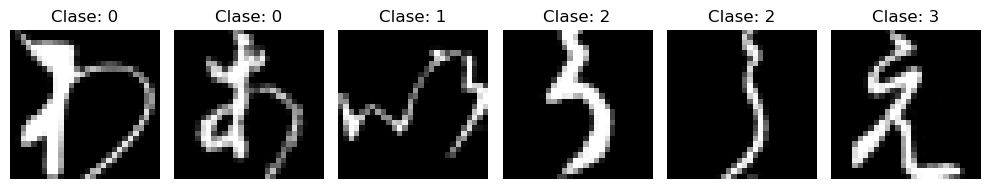
\includegraphics[width=0.9\textwidth]{figures/classes.png}
    \caption{Ejemplos de imágenes pertenecientes a distintas clases del conjunto de datos.}
    \label{fig:classes}
\end{figure}

Para entender la distribución de clases, se construyó un histograma con la cantidad de muestras por clase, mostrado en la Figura~\ref{fig:histogram}. Se observa que el dataset es balanceado, con una cantidad similar de imágenes por clase.

\begin{figure}[H]
    \centering
    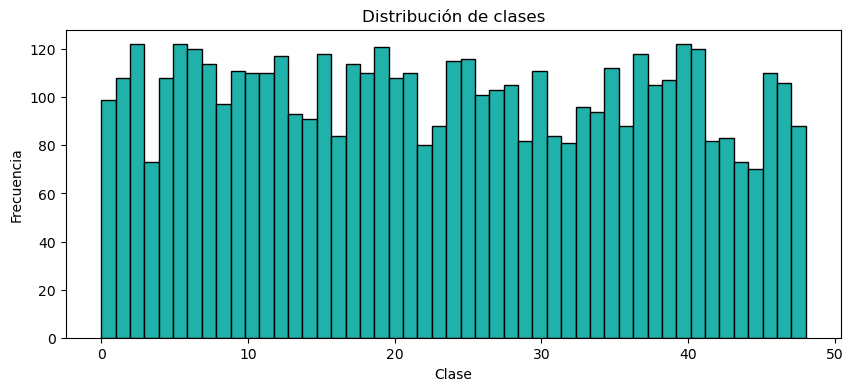
\includegraphics[width=0.9\textwidth]{figures/class_histogram.png}
    \caption{Distribución de muestras por clase en el conjunto de datos.}
    \label{fig:histogram}
\end{figure}

Las imágenes originales contienen valores enteros entre 0 y 255, correspondientes a la intensidad de gris en cada píxel. Para facilitar el entrenamiento de la red neuronal, se aplicó una normalización dividiendo todos los valores por 255, de modo que queden en el rango \([0,1]\). Esto asegura que todas las entradas tengan magnitudes comparables y evita problemas numéricos durante la propagación hacia adelante y atrás.

\subsubsection*{Particionado de los datos}

El conjunto completo fue dividido en tres subconjuntos disjuntos siguiendo la proporción:

\[
\text{Entrenamiento: } 70\%, \quad
\text{Validación: } 15\%, \quad
\text{Test: } 15\%
\]

El conjunto de entrenamiento se utilizó para el ajuste de parámetros. El conjunto de validación se empleó para la selección de hiperparámetros y monitoreo, y el conjunto de test se mantuvo completamente separado hasta el final del experimento, y se utilizó exclusivamente para la evaluación final de cada modelo entrenado.
\subsection*{Modelo Base: M0}

El modelo M0 consistió en una red neuronal feedforward con dos capas ocultas de 100 y 80 unidades respectivamente, utilizando activaciones ReLU y una capa de salida softmax para producir una distribución de probabilidad sobre las 49 clases.

Este modelo fue implementado desde cero y entrenado mediante descenso del gradiente estándar (full batch), sin utilizar regularización, optimizadores avanzados ni técnicas adicionales de estabilización.

\paragraph{Entrenamiento:} El modelo fue entrenado hasta un máximo de 5000 épocas, utilizando early stopping para finalizar automáticamente si la pérdida de validación no mejoraba durante un número determinado de épocas consecutivas. Inicialmente se adoptó esta estrategia para reducir el tiempo de entrenamiento en los experimentos, pero posteriormente se observó que también contribuía a una mejora significativa en la capacidad de generalización del modelo.

\paragraph{Resultados:}

Las métricas obtenidas durante el entrenamiento y validación del modelo se resumen en la siguiente tabla:

\begin{table}[H]
    \centering
    \begin{tabular}{lcccc}
        \hline
        Métrica & Train Loss & Train Acc & Val Loss & Val Acc \\
        \hline
        M0 & \texttt{0.8147} & \texttt{0.8097} & \texttt{1.7063} & \texttt{0.5827} \\
        \hline
    \end{tabular}
    \caption{Métricas del modelo M0 en entrenamiento y validación.}
    \label{tab:metrics-m0}
\end{table}

En la Figura~\ref{fig:plots-m0} se presentan los históricos de loss y accuracy para los conjuntos de entrenamiento y validación, así como la matriz de confusión obtenida sobre el conjunto de validation. Se observa una convergencia clara del modelo, aunque con errores frecuentes entre clases similares.

\begin{figure}[H]
    \centering
    \begin{minipage}[t]{0.32\textwidth}
        \centering
        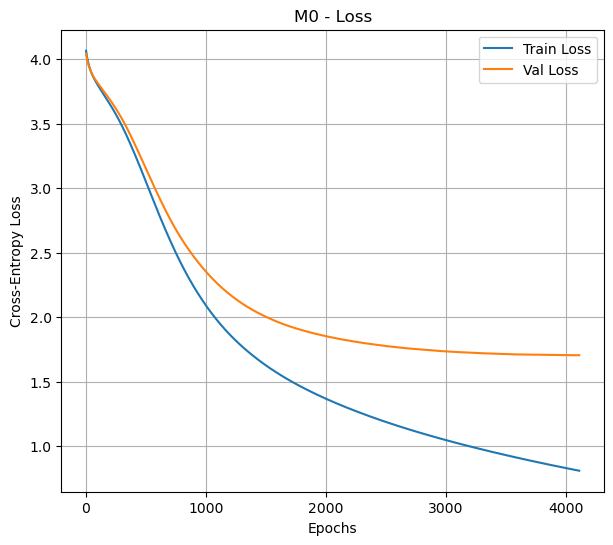
\includegraphics[width=\linewidth]{figures/loss_m0.png}
        \caption*{(a) Evolución de la pérdida.}
    \end{minipage}
    \hfill
    \begin{minipage}[t]{0.32\textwidth}
        \centering
        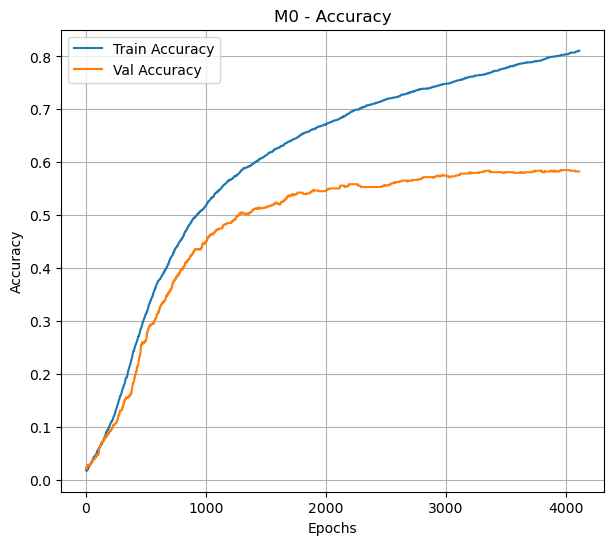
\includegraphics[width=\linewidth]{figures/acc_m0.png}
        \caption*{(b) Evolución de la precisión.}
    \end{minipage}
    \hfill
    \begin{minipage}[t]{0.32\textwidth}
        \centering
        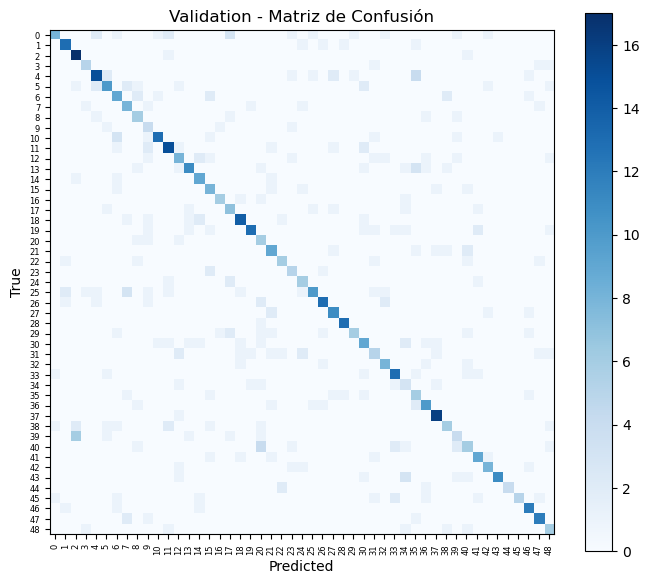
\includegraphics[width=\linewidth]{figures/conf_matrix_m0.png}
        \caption*{(c) Matriz de confusión (val).}
    \end{minipage}
    \caption{Historial de entrenamiento y matriz de confusión del modelo M0.}
    \label{fig:plots-m0}
\end{figure}

\subsection*{Modelo Mejorado: M1}

El modelo M1 partió de la misma arquitectura base que M0, pero incorporó mejoras progresivas al procedimiento de entrenamiento con el objetivo de mejorar la generalización y reducir el sobreajuste.

\paragraph{Mejoras incorporadas:}
\begin{itemize}
    \item \textbf{Mini-batch SGD:} se utilizó un tamaño de batch óptimo determinado por validación, lo cual redujo la varianza de las actualizaciones y aceleró la convergencia.
    \item \textbf{Regularización L2:} se penalizaron los pesos con un término \( \lambda \| W \|^2 \), lo que ayudó a prevenir el sobreajuste.
    \item \textbf{Early stopping:} se utilizó el mismo criterio que en M0 para detener el entrenamiento automáticamente.
    \item \textbf{Scheduler de tasa de aprendizaje:} se utilizó una reducción exponencial del learning rate a lo largo de las épocas.
    \item \textbf{Optimizador ADAM:} se reemplazó el descenso del gradiente estándar por ADAM, obteniendo una mejora significativa tanto en estabilidad como en velocidad de entrenamiento.
    \item \textbf{Dropout y BatchNorm (opcional):} se evaluaron configuraciones con y sin estas técnicas. En el modelo final se optó por incluir \texttt{AGREGAR DECISIÓN}.
\end{itemize}

La combinación de estas técnicas fue seleccionada mediante una búsqueda greedy sobre los hiperparámetros. En cada etapa se variaba únicamente un hiperparámetro, manteniendo fijos los valores óptimos encontrados hasta ese momento, y utilizando el error de validación como criterio de comparación.

Además de los hiperparámetros de entrenamiento, también se exploraron múltiples arquitecturas de red, variando tanto la cantidad de capas ocultas como la cantidad de unidades por capa. Estas pruebas permitieron encontrar estructuras que mejoraban el desempeño sin incrementar excesivamente el tiempo de entrenamiento.

El criterio de \textit{early stopping} ya utilizado en M0 fue conservado tras comprobar que, incluso al introducir nuevas mejoras, seguía representando una estrategia efectiva tanto para ahorrar tiempo de entrenamiento como para prevenir el sobreajuste.

Este enfoque progresivo fue adoptado en lugar de un grid search exhaustivo, ya que dicho método habría sido computacionalmente inviable. La búsqueda greedy permitió reducir drásticamente el número de entrenamientos necesarios, y ajustar dinámicamente los rangos de búsqueda para cada hiperparámetro sin que el costo total creciera exponencialmente.



\paragraph{Resultados:}

El modelo final seleccionado para M1 fue entrenado con las mejoras mencionadas y evaluado con los siguientes resultados:

\begin{table}[H]
    \centering
    \begin{tabular}{lcccc}
        \hline
        Métrica & Train Loss & Train Acc & Val Loss & Val Acc \\
        \hline
        M1 & \texttt{0.5740} & \texttt{0.9123} & \texttt{1.4964} & \texttt{0.6480} \\
        \hline
    \end{tabular}
    \caption{Métricas del modelo M1 en entrenamiento y validación.}
    \label{tab:metrics-m1}
\end{table}

En la Figura~\ref{fig:plots-m1} se muestra la evolución de la pérdida y precisión, junto con la matriz de confusión obtenida sobre el conjunto de validation. En comparación con M0, se observan mejores resultados, así como menor fluctuación y un entrenamiento más estable.

\begin{figure}[H]
    \centering
    \begin{minipage}[t]{0.32\textwidth}
        \centering
        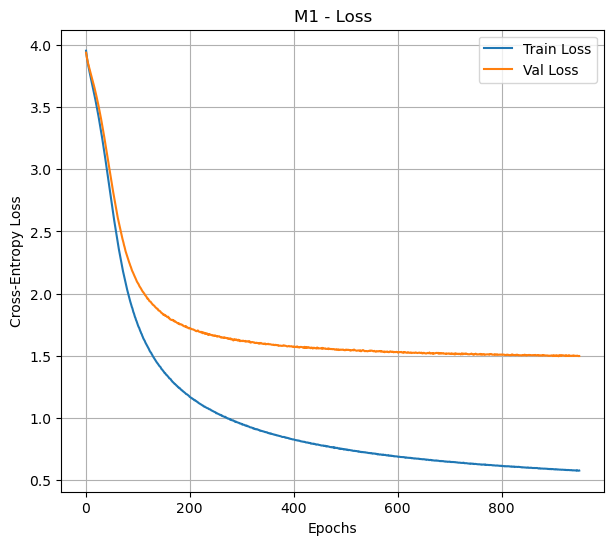
\includegraphics[width=\linewidth]{figures/loss_m1.png}
        \caption*{(a) Evolución de la pérdida.}
    \end{minipage}
    \hfill
    \begin{minipage}[t]{0.32\textwidth}
        \centering
        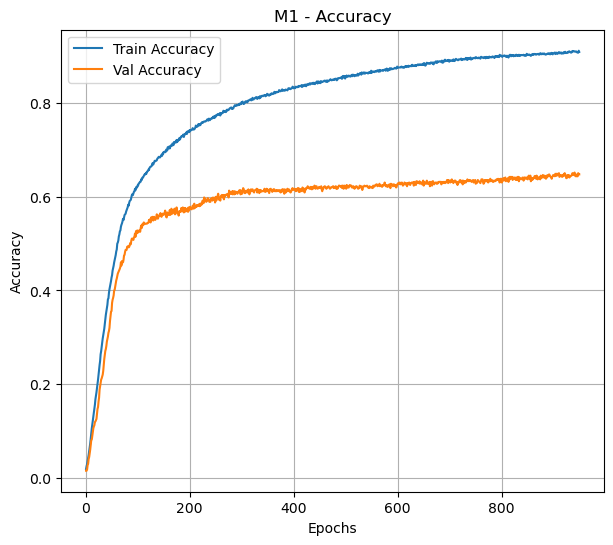
\includegraphics[width=\linewidth]{figures/acc_m1.png}
        \caption*{(b) Evolución de la precisión.}
    \end{minipage}
    \hfill
    \begin{minipage}[t]{0.32\textwidth}
        \centering
        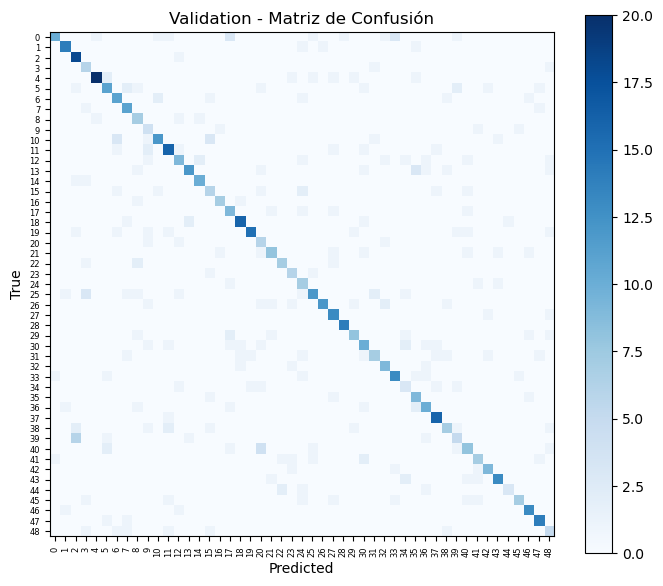
\includegraphics[width=\linewidth]{figures/conf_matrix_m1.png}
        \caption*{(c) Matriz de confusión (val).}
    \end{minipage}
    \caption{Historial de entrenamiento y matriz de confusión del modelo M1.}
    \label{fig:plots-m1}
\end{figure}

\subsection*{Modelos en PyTorch (M2, M3 y M4)}

Luego de desarrollar y evaluar los modelos con implementación propia, se decidió trasladar los experimentos a PyTorch para acelerar los tiempos de entrenamiento, facilitar la exploración de nuevas arquitecturas y aprovechar mecanismos de regularización y optimización ya implementados en el framework.

\subsubsection*{M2: Réplica del mejor modelo propio}

El modelo M2 replicó en PyTorch la mejor arquitectura e hiperparámetros obtenidos durante los experimentos con implementación propia (modelo M1). Se buscó verificar la validez de los resultados previos en un entorno de entrenamiento más eficiente y robusto.

\begin{table}[H]
    \centering
    \begin{tabular}{lcccc}
        \hline
        Métrica & Train Loss & Train Acc & Val Loss & Val Acc \\
        \hline
        M2 & \texttt{1.0854} & \texttt{0.7229} & \texttt{1.8707} & \texttt{0.5213} \\
        \hline
    \end{tabular}
    \caption{Métricas del modelo M2 en entrenamiento y validación.}
    \label{tab:metrics-m2}
\end{table}

\begin{figure}[H]
    \centering
    \begin{minipage}[t]{0.32\textwidth}
        \centering
        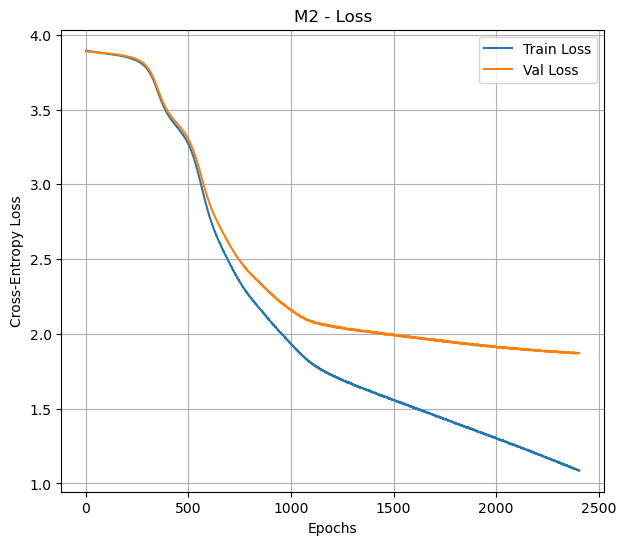
\includegraphics[width=\linewidth]{figures/loss_m2.png}
        \caption*{(a) Evolución de la pérdida.}
    \end{minipage}
    \hfill
    \begin{minipage}[t]{0.32\textwidth}
        \centering
        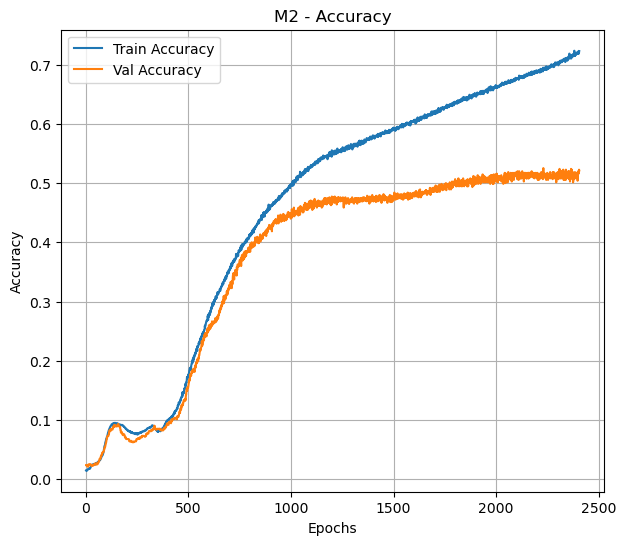
\includegraphics[width=\linewidth]{figures/acc_m2.png}
        \caption*{(b) Evolución de la precisión.}
    \end{minipage}
    \hfill
    \begin{minipage}[t]{0.32\textwidth}
        \centering
        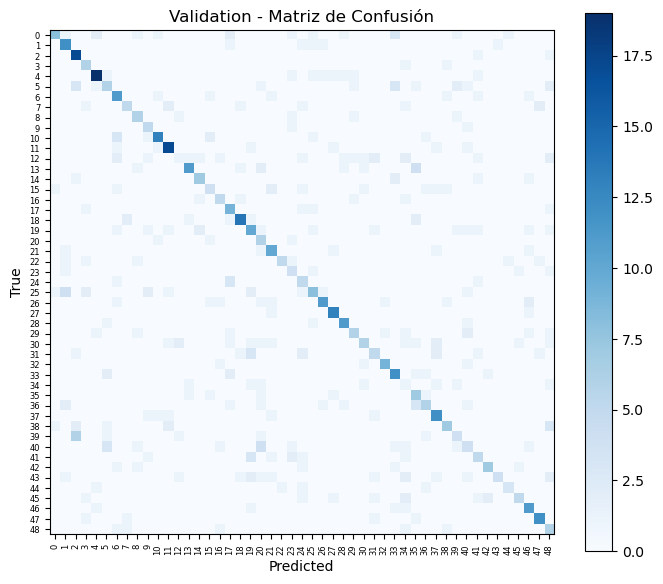
\includegraphics[width=\linewidth]{figures/conf_matrix_m2.png}
        \caption*{(c) Matriz de confusión (val).}
    \end{minipage}
    \caption{Historial de entrenamiento y matriz de confusión del modelo M2.}
    \label{fig:plots-m2}
\end{figure}

\subsubsection*{M3: Mejor arquitectura en PyTorch}

En este modelo se exploraron nuevas arquitecturas utilizando la flexibilidad de PyTorch. Se probaron variantes con mayor profundidad y distintas cantidades de unidades por capa. El modelo final seleccionado fue el que alcanzó el mejor rendimiento sobre el conjunto de validación, manteniendo un entrenamiento estable.

\begin{table}[H]
    \centering
    \begin{tabular}{lcccc}
        \hline
        Métrica & Train Loss & Train Acc & Val Loss & Val Acc \\
        \hline
        M3 & \texttt{0.9092} & \texttt{0.8286} & \texttt{1.5537} & \texttt{0.6240} \\
        \hline
    \end{tabular}
    \caption{Métricas del modelo M3 en entrenamiento y validación.}
    \label{tab:metrics-m3}
\end{table}

\begin{figure}[H]
    \centering
    \begin{minipage}[t]{0.32\textwidth}
        \centering
        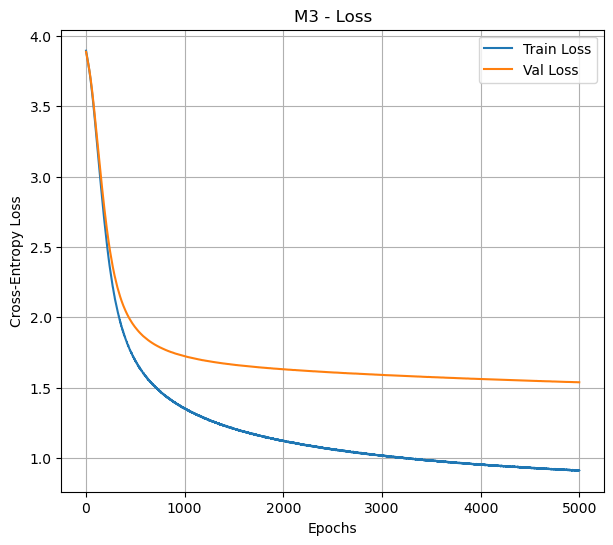
\includegraphics[width=\linewidth]{figures/loss_m3.png}
        \caption*{(a) Evolución de la pérdida.}
    \end{minipage}
    \hfill
    \begin{minipage}[t]{0.32\textwidth}
        \centering
        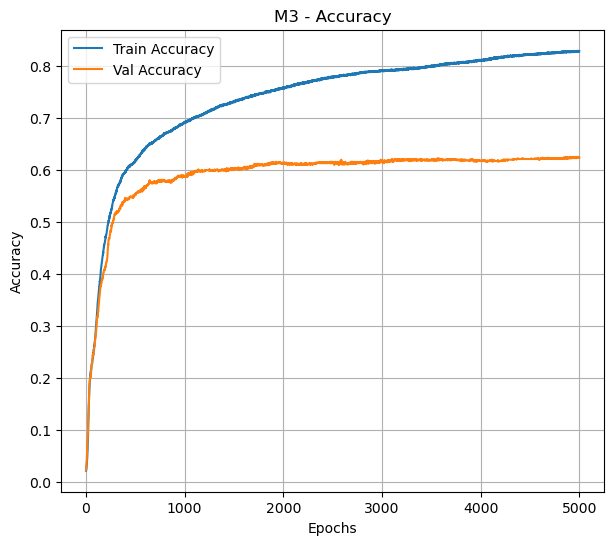
\includegraphics[width=\linewidth]{figures/acc_m3.png}
        \caption*{(b) Evolución de la precisión.}
    \end{minipage}
    \hfill
    \begin{minipage}[t]{0.32\textwidth}
        \centering
        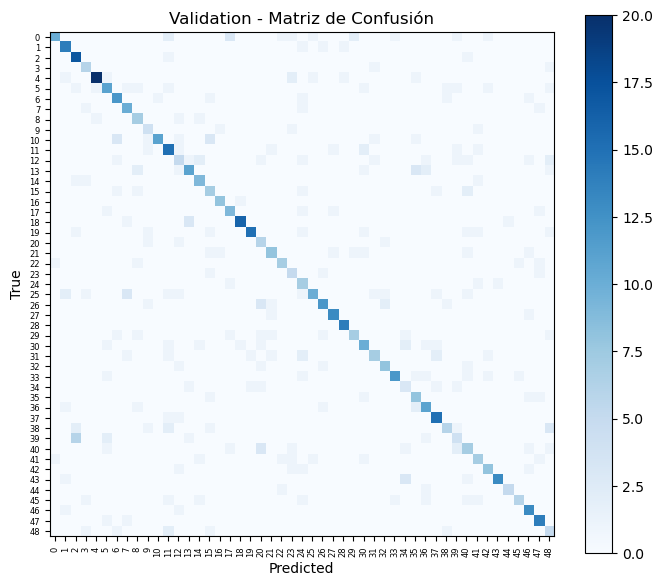
\includegraphics[width=\linewidth]{figures/conf_matrix_m3.png}
        \caption*{(c) Matriz de confusión (val).}
    \end{minipage}
    \caption{Historial de entrenamiento y matriz de confusión del modelo M3.}
    \label{fig:plots-m3}
\end{figure}

\subsubsection*{M4: Modelo con sobreajuste deliberado}

El modelo M4 fue diseñado con el objetivo de inducir un comportamiento de sobreajuste marcado, con el fin de estudiar su manifestación empírica. Para ello, se configuró una red mucho más profunda y ancha que las anteriores, con seis capas ocultas de gran tamaño: \(2048 \rightarrow 2048 \rightarrow 1024 \rightarrow 512 \rightarrow 256\). Además, se desactivaron completamente todas las técnicas de regularización: no se utilizó ni L2, ni dropout, ni batch normalization.

También se ajustaron parámetros de entrenamiento para acentuar el sobreajuste: se entrenó por 5000 épocas, sin early stopping, y utilizando un batch size muy pequeño (32) para incrementar la variabilidad del gradiente. El optimizador utilizado fue descenso por gradiente estándar, sin ADAM ni scheduler de tasa de aprendizaje.

\begin{table}[H]
    \centering
    \begin{tabular}{lcccc}
        \hline
        Métrica & Train Loss & Train Acc & Val Loss & Val Acc \\
        \hline
        M4 & \texttt{0.0003} & \texttt{1.0000} & \texttt{9.4385} & \texttt{0.4293} \\
        \hline
    \end{tabular}
    \caption{Métricas del modelo M4 en entrenamiento y validación.}
    \label{tab:metrics-m4}
\end{table}

\begin{figure}[H]
    \centering
    \begin{minipage}[t]{0.32\textwidth}
        \centering
        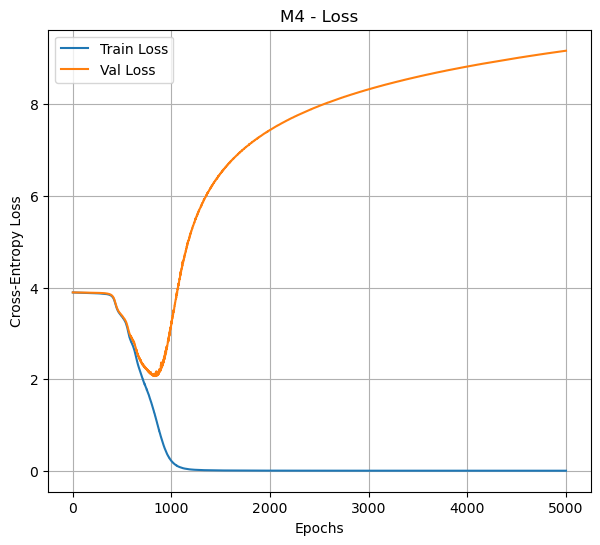
\includegraphics[width=\linewidth]{figures/loss_m4.png}
        \caption*{(a) Evolución de la pérdida.}
    \end{minipage}
    \hfill
    \begin{minipage}[t]{0.32\textwidth}
        \centering
        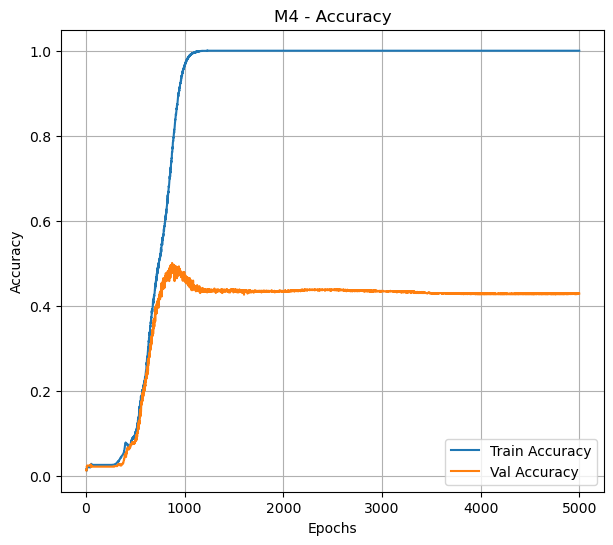
\includegraphics[width=\linewidth]{figures/acc_m4.png}
        \caption*{(b) Evolución de la precisión.}
    \end{minipage}
    \hfill
    \begin{minipage}[t]{0.32\textwidth}
        \centering
        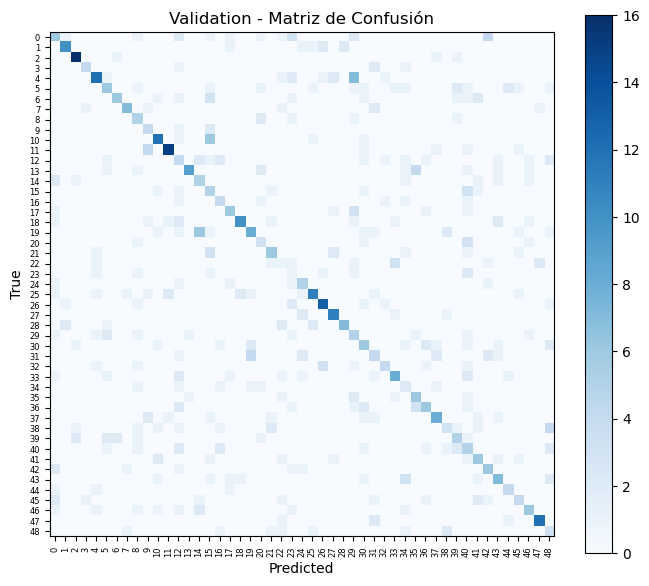
\includegraphics[width=\linewidth]{figures/conf_matrix_m4.png}
        \caption*{(c) Matriz de confusión (val).}
    \end{minipage}
    \caption{Historial de entrenamiento y matriz de confusión del modelo M4.}
    \label{fig:plots-m4}
\end{figure}

Los gráficos evidencian claramente el comportamiento típico de un modelo sobreajustado: mientras que la precisión en entrenamiento sigue aumentando y la pérdida disminuye de forma sostenida, las métricas en validación se estancan o incluso empeoran con el tiempo. La brecha creciente entre entrenamiento y validación confirma que el modelo está memorizando los datos de entrenamiento sin lograr una generalización adecuada.

\subsection*{Comparación Final de Modelos en Test}

A continuación se muestra una comparación directa del rendimiento de todos los modelos evaluados sobre el conjunto de test, considerando la métrica de accuracy, la función de pérdida (cross-entropy) y una breve observación sobre su comportamiento.

\begin{table}[H]
    \centering
    \resizebox{\textwidth}{!}{%
    \begin{tabular}{lccl}
        \toprule
        \textbf{Modelo} & \textbf{Accuracy (Test)} & \textbf{Cross-Entropy (Test)} & \textbf{Observaciones} \\
        \midrule
        M0 & \texttt{0.5800} & \texttt{1.7032} & Modelo base sin regularización \\
        M1 & \texttt{0.6427} & \texttt{1.4578} & Mejoras manuales en red propia \\
        M2 & \texttt{0.5253} & \texttt{1.9369} & PyTorch, misma arquitectura que M1 \\
        M3 & \texttt{0.6387} & \texttt{1.5455} & Mejor arquitectura general \\
        M4 & \texttt{0.4413} & \texttt{10.1525} & Sobreajuste deliberado \\

        \bottomrule
    \end{tabular}%
    }
    \caption{Comparación de métricas en test para todos los modelos evaluados.}
    \label{tab:test_comparison_models}
\end{table}

De la comparación final se observa que el modelo M1 obtuvo el mejor desempeño sobre el conjunto de test. A pesar de haber sido implementado sin frameworks externos, las mejoras incorporadas como regularización, ADAM, scheduler y early stopping permitieron lograr un equilibrio óptimo entre precisión y generalización, superando incluso a los modelos entrenados en PyTorch.

\section{Desafío: Predicción sobre conjunto oculto}

Para completar el desafío final, se utilizó el mejor modelo identificado durante el trabajo: el modelo M1, desarrollado con implementación propia. Este modelo fue aplicado sobre el conjunto de datos oculto \texttt{X\_COMP.npy}, con el objetivo de generar las probabilidades a posteriori de cada una de las 49 clases posibles.

\subsection*{Preprocesamiento y predicción}

El conjunto \texttt{X\_COMP.npy} fue cargado y normalizado del mismo modo que el resto de los datos, dividiendo todos los valores por 255 para llevarlos al rango \([0, 1]\). Luego, se utilizó el método \texttt{predict\_proba()} del modelo M1 para obtener las probabilidades asociadas a cada clase.

\subsection*{Formato de entrega}

Las predicciones generadas fueron almacenadas en un archivo \texttt{.csv} llamado:
\[\texttt{Nomberg\_Ilan\_predicciones.csv}\], siguiendo el formato requerido por el enunciado: una fila por muestra, y una columna por clase, con nombres \texttt{Clase\_0}, \texttt{Clase\_1}, ..., \texttt{Clase\_48}. Un fragmento del formato se muestra a continuación:

\begin{table}[H]
    \centering
    \begin{tabular}{cccccc}
    \toprule
    Clase\_0 & Clase\_1 & Clase\_2 & \dots & Clase\_47 & Clase\_48 \\
    \midrule
    0.8537 & 0.0000 & 1.0409 & \dots & 0.0008 & 0.0000 \\
    0.3441 & 0.0014 & 0.0002 & \dots & 0.0057 & 0.0017 \\
    0.0830 & 0.0008 & 0.0084 & \dots & 0.0045 & 0.0011 \\
    $\vdots$ & $\vdots$ & $\vdots$ & $\dots$ & $\vdots$ & $\vdots$ \\
    \bottomrule
    \end{tabular}
    \caption{Formato del archivo de salida con probabilidades por clase.}
    \label{tab:predicciones_csv}
\end{table}

\section{Conclusión}

A lo largo de este trabajo se implementaron, evaluaron y compararon distintas variantes de redes neuronales para un problema de clasificación multiclase sobre imágenes de caracteres japoneses. Se partió de un modelo base (M0) y se incorporaron mejoras progresivas (M1), cuya efectividad fue validada posteriormente mediante una implementación en PyTorch (M2–M4).

Los resultados mostraron que el modelo M1, desarrollado con implementación propia, fue el que mejor balance logró entre precisión y generalización, superando incluso a las variantes más complejas. El análisis de M4 permitió observar de forma controlada los efectos del sobreajuste, reforzando la importancia de las técnicas de regularización.

Finalmente, se utilizó el modelo M1 para generar las predicciones requeridas en el desafío final, cumpliendo con el formato especificado y demostrando la capacidad del sistema para generalizar a datos no vistos.


\end{document}




